% Chapter 2

\chapter{Compression Principles and Methods}

\label{ch:Chapter2} % For referencing the chapter elsewhere, use \autoref{ch:Chapter2}

Entropy, in essence, represents the minimal quantity of bits required to unequivocally distinguish an object within a set. Consequently, it serves as a foundational metric for the space utilization in compressed data representations. The ultimate aim of compressed data structures is to occupy space nearly equivalent to the entropy required for object identification, while simultaneously enabling efficient querying operations. This pursuit lies at the core of optimizing data compression techniques: achieving a balance between storage efficiency and query responsiveness.

\section*{Worst Case Entropy}
In its simplest form, entropy can be seen as the minimum number of bits required by identifiers (\emph{codes}, see \autoref{sec:source_and_codes}), when each element of a set $U$ has a unique code of identical length. This is called the \emph{worst case entropy} of $U$ and it's denoted by $H_{wc}(U)$. The worst case entropy of a set $U$ is given by the formula:
\begin{equation}
    H_{wc}(U) =  \log |U|
\end{equation}
where $|U|$ is the number of elements in $U$.

\begin{remark}
    If we used codes of length $l < H_{wc} (U)$, we would have only $2^l \leq 2^{H_{wc}(U)} = |U|$ possible codes, which is not enough to uniquely identify all elements in $U$.
\end{remark}

\noindent The reason behind the attribute \emph{worst case} is that if all codes are of the same length, then this length must be at least $\lceil \log |U| \rceil$ bits to be able to uniquely identify all elements in $U$. If they all have different lengths, the longest code must be at least $\lceil \log |U| \rceil$ bits long.

% \begin{example}[Worst case entropy of $\mathcal{T}_n$]
%     Let $\mathcal{T}_n$ be the set of all general ordinal trees \cite{benoit2005representing} with $n$ nodes. In this case, each node has an arbitrary number of children and distinguishes their order. Given $n$ nodes, the number of possible ordinal trees its the (n-1)-th Catalan number, which is given by the formula:
%     \begin{equation}
%         |\mathcal{T}_n| = \frac{1}{n} \binom{2n -2}{n-1}
%     \end{equation}
%     By using the Stirling approximation, we can estimate the worst case entropy of $\mathcal{T}_n$ as:
%     \begin{equation*}
%         |\mathcal{T}_n| = \frac{(2n-2)!}{n!(n-1)!} = \frac{(2n-2)^{2n-2} e^n e^{n-1}}{e^{2n-2} n^n (n-1)^{n-1} \sqrt{\pi n}} \left(1+ \left(O\frac{1}{n}\right) \right)
%     \end{equation*}
%     That is equal to $\frac{4^n}{n^{3/2}} \cdot \Theta (1)$, therefore
%     \begin{equation}
%         H_{wc} (\mathcal{T}_n) = \log | \mathcal{T}_n | = 2n - \Theta(\log n)
%     \end{equation}
%     We have then found the minimum numbers of bits required to uniquely identify (\emph{encode}) a general ordinal tree with $n$ nodes.
% \end{example}
\begin{example}[Worst-case entropy of $\mathcal{T}_n$]
    Let $\mathcal{T}_n$ denote the set of all general ordinal trees \cite{benoit2005representing} with $n$ nodes. In this scenario, each node can have an arbitrary number of children, and their order is distinguished. With $n$ nodes, the number of possible ordinal trees is the $(n-1)$-th Catalan number, given by:
    \begin{equation}
        |\mathcal{T}_n| = \frac{1}{n} \binom{2n - 2}{n - 1}
    \end{equation}
    Using Stirling's approximation, we can estimate the worst-case entropy of $\mathcal{T}_n$ as:
    \begin{equation*}
        |\mathcal{T}_n| = \frac{(2n-2)!}{n!(n-1)!} = \frac{(2n-2)^{2n-2} e^n e^{n-1}}{e^{2n-2} n^n (n-1)^{n-1} \sqrt{\pi n}} \left(1+ O\left(\frac{1}{n}\right)\right)
    \end{equation*}
    This simplifies to $\frac{4^n}{n^{3/2}} \cdot \Theta (1)$, hence
    \begin{equation}
        H_{wc} (\mathcal{T}_n) = \log |\mathcal{T}_n| = 2n - \Theta(\log n)
    \end{equation}
    Thus, we have determined the minimum number of bits required to uniquely identify (encode) a general ordinal tree with $n$ nodes.
\end{example}



\section{Entropy} \label{sec:shannon_entropy}

We now introduce the concept of entropy as a measure of uncertainty of a random variable. While the worst-case entropy $H_{wc}$, discussed previously, provides a lower bound based solely on the set's cardinality (effectively assuming fixed-length codes or a uniform probability distribution over the elements), Shannon entropy offers a more refined measure. It accounts for the actual probability distribution of the elements, quantifying the \emph{average} uncertainty or information content associated with the random variable. A deeper explanation can be found in standard texts such as \cite{han2002mathematics,navarro2016compact,ElementsofInformationTheory}.

\begin{definition}[Entropy of a Random Variable]\label{def:entropy}
    Let $X$ \marginpar{This is also known as Shannon entropy, named after Claude Shannon, who introduced it in his seminal work \cite{Shannon1948}}be a random variable taking values in a finite alphabet $\mathcal{X}$ with the probabilistic distribution $P_X(x)= \text{Pr}\{X=x\}~(x\in\mathcal{X})$. Then, the entropy of $X$ is defined as
    \begin{equation*}
        H(X) = H(P_X) \myeq E_{P_x} \{-\log P_X(x)\} = -\sum_{x\in\mathcal{X}} P_X(x)\log P_X(x)
    \end{equation*}
\end{definition}
Here, $E_{P_X}[\cdot]$ denotes the expectation with respect to the probability distribution $P_X$. The logarithm is taken to base 2, and entropy is expressed in bits. From the definition, it follows that the entropy of a discrete random variable is always non-negative\footnote{The entropy is zero if and only if $X$ is deterministic, i.e., $P_X(x)=1$ for some single value $x=c$.}. \label{foot:entropy_nonneg}.

\begin{example}[Toss of a fair coin]
    Let $X$ be a random variable representing the outcome of a fair coin toss, with $\mathcal{X}=\{Heads, Tails\}$. The probability distribution is $P_X(\text{Heads}) = P_X(\text{Tails}) = \frac{1}{2}$. The entropy of $X$ is:
    \begin{equation*}
        H(X) = -\frac{1}{2}\log_2\frac{1}{2} - \frac{1}{2}\log_2\frac{1}{2} = -\frac{1}{2}(-1) - \frac{1}{2}(-1) = 1 \text{ bit}
    \end{equation*}
    This result aligns with the intuition that one bit is required to convey the outcome of a fair coin toss.
\end{example}

\begin{remark}
    By convention, $H(X)$ denotes the entropy of the random variable $X$. It is important to note that entropy is not a function of the random variable itself, but rather a functional of its probability distribution $P_X$. It depends only on the probabilities of the values, not the values themselves.
\end{remark}

The entropy $H(X)$ quantifies the average uncertainty associated with the random variable $X$. It can be interpreted as the average amount of information (in bits) gained upon observing an outcome of $X$, or equivalently, the minimum average number of bits required to encode the outcomes of $X$ using an optimal compression scheme.

\subsection{Properties}
Having introduced the entropy for a single random variable $X$, we now consider the case of two random variables $X$ and $Y$. To quantify the total uncertainty associated with the pair $(X,Y)$ considered together, we define the joint entropy:

\begin{definition}[Joint Entropy]\label{def:joint_entropy}
    Let $(X,Y)$ be a pair of discrete random variables $(X,Y)$ with a joint distribution $P_{XY}(x,y) = \text{Pr}\{X=x,Y=y\}$. The joint entropy of $(X,Y)$ is defined as
    \begin{equation*}\label{eq:joint_entropy}
        H(X,Y) = H(P_{XY}) = -\sum_{x\in\mathcal{X}}\sum_{y\in\mathcal{Y}} P_{XY}(x,y)\log P_{XY}(x,y)
    \end{equation*}
\end{definition}
This definition extends naturally to the joint entropy of $n$ random variables $(X_1,X_2,\ldots,X_n)$ as $H(X_1,\ldots, X_n)$.

We also define the conditional entropy $H(Y|X)$, which measures the remaining uncertainty about $Y$ when $X$ is known. It is the expected value of the entropies of the conditional distributions $P_{Y|X}(y|x)$, averaged over $X$.

Often, it's helpful to conceptualize the relationship between $Y$ and $X$ in terms of information transmission. Given $X=x$, the conditional probability $P_{Y|X}(y|x) = \text{Pr}\{Y=y|X=x\}$ describes the likelihood of observing $Y=y$. The collection of these conditional probabilities for all $x \in \mathcal{X}$ and $y \in \mathcal{Y}$ defines a statistical relationship often referred to as a \emph{channel} with \emph{input alphabet} $\mathcal{X}$ and \emph{output alphabet} $\mathcal{Y}$.

\begin{definition}[Conditional Entropy]\label{def:conditional_entropy}
    Let $(X,Y)$ be a pair of discrete random variables with a joint distribution $P_{XY}(x,y) = \text{Pr}\{X=x,Y=y\}$. The conditional entropy of $Y$ given $X$ is defined as
    \begin{align*}
        H(Y|X) & = H(W | P_X) \myeq \sum_x P_X(x)H(Y|x)                                                       \\
               & = \sum_{x \in \mathcal{X}} P_X(x) \Big\{ -\sum_{y \in \mathcal{Y}} W(y|x) \log W(y|x) \Big\} \\
               & = -\sum_{x\in\mathcal{X}}\sum_{y\in\mathcal{Y}} P_{XY}(x,y)\log W(y|x)                       \\
               & = E_{P_{XY}} \{ -\log W(Y|X) \}
    \end{align*}
\end{definition}

Since entropy is non-negative, and $H(Y|X)$ is an average of non-negative entropies $H(Y|X=x)$, conditional entropy is also non-negative: $H(Y|X) \ge 0$. Furthermore, $H(Y|X) = 0$ if and only if $Y$ is completely determined by $X$ (i.e., $Y=f(X)$ for some deterministic function $f$ with probability one).

The relationship between joint and conditional entropy is established by the chain rule.

\begin{theorem}[Chain Rule]\label{thm:chain_rule}
    Let $(X,Y)$\marginpar{This is also known as additivity of entropy.} be a pair of discrete random variables with a joint distribution $P_{XY}(x,y)$. Then, the joint entropy of $(X,Y)$ can be expressed as
    \begin{equation*}
        H(X,Y) = H(X) + H(Y|X)
    \end{equation*}
\end{theorem}
\begin{proof}
    From the definition of conditional entropy (\ref{def:conditional_entropy}), we have
    \begin{align*}
        H(X,Y) & = -\sum_{x,y} P_{XY}(x,y) \log W(y|x)                                        \\
               & = -\sum_{x,y} P_{XY}(x,y) \log \frac{P_{XY}(x,y)}{P_X(x)}                    \\
               & = -\sum_{x,y} P_{XY}(x,y) \log P_{XY}(x,y) + \sum_{x,y} P_{X}(x) \log P_X(x) \\
               & = H(X,Y) + H(X)
    \end{align*}
    Where we used the relation
    \begin{equation*}
        W(y|x) = \frac{P_{XY}(x,y)}{P_X(x)}
    \end{equation*}
    When $P_X(x) \neq 0$.
\end{proof}

\begin{corollary}
    \begin{equation*}
        H(X, Y|Z) = H(X|Z) + H(Y|X,Z)
    \end{equation*}
\end{corollary}
\begin{proof}
    The proof is analogous to the proof of the chain rule.
\end{proof}

\begin{corollary}
    \begin{align*}
        H(X_1, X_2, \ldots, X_n) & = H(X_1) + H(X_2|X_1) + H(X_3|X_1, X_2) \nonumber \\
                                 & + \ldots + H(X_n|X_1, X_2, \ldots, X_{n-1})
    \end{align*}
\end{corollary}
\begin{proof}
    We can apply the two-variable chain rule in repetition obtain the result.
\end{proof}

\subsection{Mutual Information}
Having defined measures for the uncertainty of individual variables ($H(X)$), pairs ($H(X,Y)$), and conditional uncertainty ($H(Y|X)$), we can quantify the amount of information that one variable provides about another. This is the mutual information, $I(X;Y)$. It represents the reduction in uncertainty about $X$ obtained by learning the value of $Y$, or vice versa. Figure \ref{fig:mutual_information} provides a visual representation.

\begin{definition}[Mutual Information]\label{def:mutual_information}
    Let $(X,Y)$ be a pair of discrete random variables with a joint distribution $P_{XY}(x,y)$. The mutual information between $X$ and $Y$ is defined as
    \begin{equation}
        I(X;Y) = H(X) - H(X|Y)
    \end{equation}
\end{definition}
Using the chain rule (\ref{thm:chain_rule}), we can rewrite it as
\begin{align}
    I(X;Y) & = H(X) - H(X|Y) \nonumber                                           \\
           & = H(X) + H(Y) - H(X,Y)                                              \\
           & = -\sum_x P_X(x)\log P_X(x) - \sum_y P_Y(y)\log P_Y(y) \nonumber    \\
           & \quad + \sum_{x,y} P_{XY}(x,y)\log P_{XY}(x,y)                      \\
           & = \sum_{x,y} P_{XY}(x,y)\log \frac{P_{XY}(x,y)}{P_X(x)P_Y(y)}       \\
           & = E_{P_{XY}} \left\{ \log \frac{P_{XY}(x,y)}{P_X(x)P_Y(y)} \right\}
\end{align}
It follows immediately that the mutual information is symmetric, $I(X;Y) = I(Y;X)$.

\begin{figure}[h!]
    \centering
    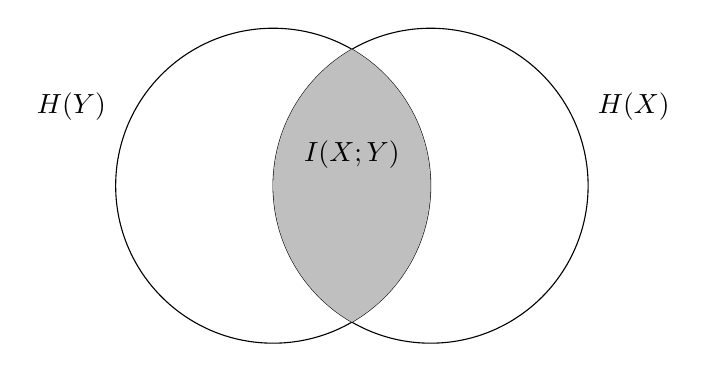
\begin{tikzpicture}
        % Define the circles
        \def\radius{2cm}
        \def\dist{2cm}
        \coordinate (center1) at (0,0);
        \coordinate (center2) at (\dist,0);

        % Draw circles
        \draw (center1) circle [radius=\radius];
        \draw (center2) circle [radius=\radius];

        % Color intersection
        \begin{scope}
            \clip (center1) circle (\radius);
            \fill[lightgray] (center2) circle (\radius);
        \end{scope}

        % Label intersection
        \coordinate (intersection) at (\dist/2,0);
        \node at (intersection) [below, above=0.1cm] {$I(X;Y)$};

        % Move labels outside
        \node at (center1) [above=1cm, left=2cm] {$H(Y)$};
        \node at (center2) [above=1cm, right=2cm] {$H(X)$};
    \end{tikzpicture}
    \caption{Mutual information between two random variables $X$ and $Y$.\label{fig:mutual_information}}
\end{figure}

\subsection{Fano's inequality}

Information theory provides fundamental limits on data processing tasks, including compression and inference. It allows us to establish lower bounds on the probability of error when estimating one random variable based on observations of another. Fano's inequality relates the conditional entropy $H(X|Y)$ to the probability of error when estimating $X$ from $Y$. Recall that $H(X|Y) = 0$ if and only if $X$ is a function of $Y$, meaning $X$ can be determined from $Y$ with zero error. Fano's inequality bounds the error probability when $H(X|Y) > 0$.

\begin{theorem}[Fano's Inequality]\label{thm:fano_inequality}
    Let $X$ and $Y$ be two discrete random variables with $X$ taking values in some discrete alphabet $\mathcal{X}$, we have
    \begin{equation*}
        H(X|Y) \leq \text{Pr}\{X \neq Y\} \log (|\mathcal{X}|-1) + h(\text{Pr}\{X \neq Y\})
    \end{equation*}
    where $h(p) = -p\log p - (1-p)\log(1-p)$ is the binary entropy function.
\end{theorem}
\begin{proof}
    Let $Z$ be a random variable defined as follows:
    \begin{equation*}\label{eq:random_variable_Z}
        Z = \begin{cases}
            1 & \text{if } X \neq Y \\
            0 & \text{if } X = Y
        \end{cases}
    \end{equation*}
    We can then write
    \begin{align} \label{eq:entropy_decomposition}
        H(X|Y) & = H(X|Y) + H(Z|XY) = H(XZ|Y) \nonumber \\
               & = H(X|YZ) + H(Z|Y) \nonumber           \\
               & \leq H(X|YZ) + H(Z)
    \end{align}
    The last inequality follows from the fact that conditioning reduces entropy. We can then write
    \begin{equation} \label{eq:entropy_decomposition2}
        H(Z) = h(\text{Pr}\{X \neq Y\})
    \end{equation}
    Since $\forall y \in \mathcal{Y}$, we can write
    \begin{equation*}
        H(X | Y =y, Z =0) =0
    \end{equation*}
    and
    \begin{equation*}
        H(X| Y = y, Z = 1) \leq \log(|\mathcal{X}|-1)
    \end{equation*}
    Combining these results, we have
    \begin{equation} \label{eq:entropy_decomposition3}
        H(X | YZ) \leq \text{Pr}\{X \neq Y\} \log (|\mathcal{X}|-1)
    \end{equation}
    From equations \ref{eq:entropy_decomposition}, \ref{eq:entropy_decomposition2} and \ref{eq:entropy_decomposition3}, we have Fano's inequality.
\end{proof}
Fano's inequality thus provides a tangible link between the conditional entropy $H(X|Y)$, which quantifies the remaining uncertainty about $X$ when $Y$ is known, and the minimum probability of error achievable in any attempt to estimate $X$ from $Y$. This inequality, along with the foundational concepts of entropy, joint entropy, conditional entropy, and mutual information introduced throughout this section, establishes a robust theoretical framework. These tools are not merely abstract measures; they allow us to quantify information, understand dependencies between data sources, and ultimately, to delineate the fundamental limits governing how efficiently data can be represented and compressed. Understanding these limits is essential as we go deeper into specific encoding techniques.

\section{Source and Code} \label{sec:source_and_codes}

TODO: Some introduction about the source and coding, maybe with some very simple example like the morse code that uses a single dot to represent the most common symbol.

% We enrich the understanding of entropy by establishing its core role in setting the fundamental limit for information compression. This process involves condensing data by assigning shorter descriptions to more frequent outcomes and longer descriptions to less frequent ones. For example, Morse code uses a single dot to represent the most common symbol. Within this chapter, we ascertain the minimum average description length for a random variable. \cite{ElementsofInformationTheory}

\subsection{Codes}

A source characterized by a random process generates symbols from a specific alphabet at each time step. The objective is to transform this output sequence into a more concise representation. This data reduction technique, known as \emph{source coding} or \emph{data compression}, utilizes a code to represent the original symbols more efficiently. The device that performs this transformation is termed an \emph{encoder}, and the process itself is referred to as \emph{encoding}. \cite{han2002mathematics}

\begin{definition}[Source Code]\label{def:code}
    A source code for a random variable $X$ is a mapping from the set of possible outcomes of $X$, called $\mathcal{X}$, to $\mathcal{D}^*$, the set of all finite-length strings of symbols from a $\mathcal{D}$-ary alphabet. Let $C(X)$ denote the codeword assigned to $x$ and let $l(x)$ denote length of $C(x)$
\end{definition}

\begin{definition}[Expected length]\label{def:expected_length}
    The expected length $L(C)$ of a source code $C$ for a random variable $X$ with probability mass function $P_X(x)$ is defined as
    \begin{equation}
        L(C) = \sum_{x\in\mathcal{X}} P_X(x)l(x)
    \end{equation}
    where $l(x)$ is the length of the codeword assigned to $x$.
\end{definition}

\noindent Let's assume from now for simplicity that the $\mathcal{D}$-ary alphabet is $\mathcal{D} = \{0, 1, \ldots, D-1\}$.

\begin{example}
    Let's consider a source code for a random variable $X$ with $\mathcal{X} = \{a, b, c, d\}$ and $P_X(a) = 0.5$, $P_X(b) = 0.25$, $P_X(c) = 0.125$ and $P_X(d) = 0.125$. The code is defined as
    \begin{align*}
        C(a) &= 0 \\
        C(b) &= 10 \\
        C(c) &= 110 \\
        C(d) &= 111
    \end{align*}
    The entropy of $X$ is
    \begin{equation*}
        H(X) = 0.5\log 2 + 0.25\log 4 + 0.125\log 8 + 0.125\log 8 = 1.75 \text{ bits}
    \end{equation*}
    The expected length of this code is also $1.75$:
    \begin{equation*}
        L(C) = 0.5 \cdot 1 + 0.25 \cdot 2 + 0.125 \cdot 3 + 0.125 \cdot 3 = 1.75 \text{ bits}
    \end{equation*}
    In this example we have seen a code that is optimal in the sense that the expected length of the code is equal to the entropy of the random variable.
\end{example}

\begin{example}[Morse Code]\label{ex:morse_code}
    TODO from \cite{ElementsofInformationTheory}
\end{example}

\begin{definition}[Nonsingular Code]\label{def:nonsingular_code}
    TODO from \cite{ElementsofInformationTheory}
\end{definition}

\begin{definition}[Extension of a Code]\label{def:extension_code}
    TODO from \cite{ElementsofInformationTheory}
\end{definition}

\begin{definition}[Unique Decodability]\label{def:unique_decodability}
    TODO from \cite{ElementsofInformationTheory}
\end{definition}

\begin{definition}[Prefix Code]\label{def:prefix_code}
    TODO from \cite{ElementsofInformationTheory}
\end{definition}

TODO: Add a paragraph about the fact that  Shannon entropy provides a lower bound for the average length of a uniquely decodable code. (For example for \cite{KolmogorovComplexity} 7.1.2)

\subsection{Kraft's Inequality}

Some introduction from \cite{ElementsofInformationTheory}

\begin{theorem}[Kraft's Inequality]\label{thm:kraft_inequality}
    TODO from \cite{ElementsofInformationTheory}
\end{theorem}
\begin{proof}
    TODO from \cite{ElementsofInformationTheory}
\end{proof}

\subsection{Source Coding Theorem}

Some introduction from \cite{ElementsofInformationTheory,Shannon1948,KolmogorovComplexity,han2002mathematics}

\begin{theorem}[Source Coding Theorem]\label{thm:source_coding_theorem}
    TODO from \cite{ElementsofInformationTheory,han2002mathematics}
\end{theorem}
\begin{proof}
    TODO from \cite{ElementsofInformationTheory,han2002mathematics}
\end{proof}







\clearpage


\section{Empirical Entropy}
Before digging into the concept of empirical entropy, let's begin with the notion of binary entropy. Consider an alphabet $\mathcal{U}$, where $\mathcal{U} = \{0, 1\}$. Let's assume it emits symbols with probabilities $p_0$ and $p_1 = 1 - p_0$. The entropy of this source can be calculated using the formula:
\[
H(p_0) = -p_0 \log_2 p_0 - (1 - p_0) \log_2 (1 - p_0)
\]
We can extend this concept to scenarios where the elements are no longer individual bits, but sequences of these bits emitted by the source. Initially, let's assume the source is \emph{memoryless} (or \emph{zero-order}), meaning the probability of emitting a symbol doesn't depend on previously emitted symbols. In this case, we can consider chunks of $n$ bits as our elements. Our alphabet becomes $\Sigma = \{0, 1\}^n$, and the Shannon Entropy of two independent symbols $x, y \in \Sigma$ will be the sum of their entropies. Thus, if the source emits symbols from an alphabet $\Sigma = [0,\sigma]$ where each symbol has a probability $p_s$, the entropy of the source becomes:

\[
H(p_1, \ldots, p_{\sigma}) = - \sum_{s=1}^{\sigma} p_s \log p_s = \sum_{s=1}^{\sigma} p_s \log \frac{1}{p_s}
\]

\begin{remark}
    If all symbols have a probability of $p_s =1$, then the entropy is $0$, and all other probabilities are $0$. If all symbols have the same probability $\frac{1}{\sigma}$, then the entropy is $\log \sigma$. So given a sequence of $n$ elements from an alphabet $\Sigma$, belonging to $\mathcal{U} = \Sigma^n$, its entropy is straightforwardly $n \mathcal{H}(p_1, \ldots, p_{\sigma})$
\end{remark}

% \noindent This approach however relies on the assumption that individual sequences originate from a single source. Let's consider relaxing this assumption and explore how Shannon Entropy can be used to define an entropy concept for text.

\subsection{Bit Sequences}
Let's consider a bit sequence, $B[1, n]$, which we aim to compress without access to an explicit model of a known bit source. Instead, we only have access to $B$. Although lacking a precise model, we may reasonably anticipate that B exhibits a bias towards either more $0s$ or more $1s$. Hence, we might attempt to compress $B$ based on this characteristic. Specifically, we say that $B$ is generated by a zero-order source emitting $0s$ and $1s$. Assuming $m$ represents the count of $1s$ in $B$, it's reasonable to posit that the source emits $1s$ with a probability of $p = m/n$. This leads us to the concept of zero-order empirical entropy:

\begin{definition}[Zero-order empirical entropy]
    Given a bit sequence $B[1, n]$ with $m$ $1s$ and $n-m$ $0s$, the zero-order empirical entropy of $B$ is defined as:
   \begin{equation}
     \mathcal{H}_0(B) = \mathcal{H} \left( \frac{m}{n} \right) =\frac{m}{n} \log \frac{n}{m} + \frac{n-m}{n} \log \frac{n}{n-m}
   \end{equation}
\end{definition}
\noindent The concept of zero-order empirical entropy carries significant weight: it indicates that if we attempt to compress $B$ using a fixed code $C(1)$ for $1s$ and $C(0)$ for $0s$, then it's impossible to compress $B$ to fewer than $\mathcal{H}_0(B)$ bits per symbol. Otherwise, we would have $m |C(1)| + (n-m) |C(0)| < n \mathcal{H}_0(B)$, which violates the lower bound established by Shannon entropy.

\paragraph{Connection with worst case entropy}
TBD if to add this paragraph, from \cite{navarro2016compact} 2.3.1

\subsection{Entropy of a Text}
The zero-order empirical entropy of a string $S[1, n]$, where each symbol $s$ occurs $n_s$ times in $S$, is similarly determined by the Shannon entropy of its observed probabilities:
\begin{definition}[Zero-order empirical entropy of a text]
    Given a text $S[1, n]$ with $n_s$ occurrences of symbol $s$, the zero-order empirical entropy of $S$ is defined as:
    \begin{equation}
        \mathcal{H}_0(S) = \mathcal{H} \left( \frac{n_1}{n} , \ldots, \frac{n_{\sigma}}{n} \right) =  \sum_{s=1}^{\sigma} \frac{n_s}{n} \log \frac{n}{n_s}
    \end{equation}
\end{definition}
\begin{example}
    TODO: Classic example on finding the zero-order empirical entropy of a word like abracadabra or banana
\end{example}
However, this definition falls short because in most natural languages, symbol choices aren't independent. For example, in English text, the sequence "\emph{don'}" is almost always followed by "\emph{t}". Higher-order entropy (section \ref{sec:higher_order_entropy}) is a more accurate measure of the entropy of a text, as it considers the probability of a symbol given the preceding symbols

\clearpage
\section{Higher Order Entropy} \label{sec:higher_order_entropy}

TODO: A bit of introduction
\begin{definition}[Redundacy] \label{def:redundancy}
    TODO: Give a formal definition of redundacy: informally is a measure of the distance between the source's entropy and the compression ration, and can thereby be seen as a measure of how fast the algorithm reaches the entropy of the source.
\end{definition}

% All these measures are very interesting, but unrealistic because it's quite unusual, if not impossibile, to know the entropy of the soCompression applications employ a wide variety of techniques and have quite different degrees of
complexity, but share some common processeurce that generate the stringe we are going to compress. In order to circumvent this problem, a different empirical approach has been taken by introducing the notion of \emph{k-th order empirical entropy} of a string $S$, denoted by $\mathcal{H}_k(S)$. In \ref{sec:statistical_coding} we have discussed the case where $k=0$, which depends on the frequency of the symbols in the string. Here, we wish with $\mathcal{H}_k(S)$ to empower the entropy definition by considering the frequencies ok $k$-grams in the string $S$, thus taking into account subsequences of symbols of length $k$, hence the \emph{compositional structure} of $S$

\noindent While using measures like \ref{def:redundancy} are certainly intriguing, their actual usability is questionable due to the inherent challenge of determining the entropy of the source generating the string we aim to compress. To address this issue, an alternative empirical approach is the concept of the \emph{k-th order empirical entropy} of a string $S$, denoted as $\mathcal{H}_k(S)$. In statistical coding (\autoref{sec:statistical_coding}), we will see a scenario where $k=0$, relying on symbol frequencies within the string. Now, with $\mathcal{H}_k(S)$, our objective is to extend the entropy concept by examining the frequencies of $k$-grams in string $S$. This requires analyzing subsequences of symbols with a length of $k$, thereby capturing the \emph{compositional structure} of $S$. \cite{ferragina2023pearls} \vspace{0.4cm}

\noindent Let $S$ be a string over the alphabet $\Sigma=\{\sigma_1, \dots, \sigma_n\}$. Denote with $n_\omega$ the number of occurrences of the $k$-gram $\omega$ in $S$. \footnote{We will use the notation $\omega \in \Sigma^k$ to denote a $k$-gram, i.e., a subsequence of $k$ symbols in the string $S$.}

\begin{definition}[k-th Order Empirical Entropy] \label{def:kth_order_empirical_entropy}
    The \emph{k-th order empirical entropy} of a string $S$ is defined as
    \begin{equation}
        \mathcal{H}_k(S) = \frac{1}{|S|} \sum_{\omega \in \Sigma^k} \left ( \sum_{i=1}^h n_{\omega\sigma_i} \log \left ( \frac{n_\omega}{n_{\omega\sigma_i}} \right) \right )
    \end{equation}
    where $|S|$ is the length of the string $S$.
\end{definition}

\noindent When considering a sequence $S[1,n]$ we can compute the \emph{empirical k-th entropy} of $S$ by considering the frequencies of symbols depending on the $k$ preceding symbols.
\begin{equation}
    \mathcal{H}_k(S) = \sum_{\omega \in \Sigma^k} \frac{|S_\omega|}{n} \cdot \mathcal{H_0}(S_\omega)
\end{equation}
where $S_\omega$ is a string formed by collecting the symbol that follows each occurrence of the $k$-gram $\omega = \sigma_1 \dots \sigma_k$ in $S$.

\begin{example}
    Consider the example \ref{ex:0_order_entropy_abracadabra}, where $S = \text{"abracadabra"}$ and $\Sigma = \{a, b, c, d, r\}$. The zero-order empirical entropy of $S$ is $\mathcal{H}_0(S) \approx 2.04$. Now, let's calculate the first-order empirical entropy of $S$. We have that $S_a = \text{"bcdb\$"}$ (where $\$$ is the end-of-string symbol), $S_b = \text{"rr"}$, $S_c = \text{"a"}$, $S_d = \text{"a"}$, and $S_r = \text{"aa"}$. Thus, $H_0(S_a) \approx 1.922$, $H_0(S_b) = H_0(S_c) = H_0(S_d) = H_0(S_r) = 0$. Therefore, the first-order empirical entropy of $S$ is:
    \[
        \mathcal{H}_1(S) = \frac{5}{11} \cdot \mathcal{H}_0(S_a) \approx 0.874
    \]
    That is much lower than the zero-order empirical entropy of $S$.
\end{example}

\noindent The quantity $n \mathcal{H}_k(S)$ serves as a lower bound for the minimum number of bits attainable by any encoding of $S$, under the condition that the encoding of each symbol may rely on itself and the $k$ symbols preceding it in $S$. Consistently, any compressor that surpasses this threshold would also have the capability to compress symbols originating from the related $k$th-order source to a level lower than its Shannon entropy.

\begin{remark}
    % For large values of $k$ (at most $k=n-1$), and usually sooner) the $k$-th order empirical entropy of $S$ is null since all the $k$-grams appear only once. If we arrive at this point, our model becomes useless as a lower bound for compressors. Even before reaching the value $k$ for which $\mathcal_k(S)=0$, compressors cannot achieve $n\mathcal_k(S)$ bits in practice for very high $k$ values, because they must store the set of $\sigma^{k+1}$ probabilities, or equivalently, the set of $\sigma^{k+1}$ codes\footnote{Similarly, adaptive compressor must record $\sigma^{k+1}$, escape symbols somewhere along the compressed file}, so that the decompressor can reconstruct $S$. In theory, it is common to assume that $S$ can be compressed up to $n \mathcal{H}_k(S) + o(n)$ bits for any $k+1 \leq \alpha log_\sigma n$ and any constant $0 < \alpha < 1$, because in this case one can store $\sigma^{k+1}$ numbers in $[1,n]$ (such as the frequencies of the $k$-grams) within $\sigma^{k+1} \log n \leq n^\alpha log n = o(n)$ bits. \cite{navarro2016compact}
    As $k$ grows large (up to $k=n-1$, and often sooner), the $k$-th order empirical entropy of $S$ reaches null, given that each $k$-gram appears only once. This renders our model ineffective as a lower bound for compressors. Even before reaching the $k$ value where $\mathcal{H}_k(S)=0$, compressors face practical difficulties in achieving the target of $n\mathcal{H}_k(S)$ bits, particularly for high $k$ values. This is due to the necessity of storing the set of $\sigma^{k+1}$ probabilities or codes, adding complexity to compression. Likewise, adaptive compressors must incorporate $\sigma^{k+1}$ escape symbols into the compressed file, further complicating the process. In theory, it is commonly assumed that $S$ can be compressed up to $n \mathcal{H}k(S) + o(n)$ bits for any $k+1 \leq \alpha \log\sigma n$ and any constant $0 < \alpha < 1$. In such cases, storing $\sigma^{k+1}$ numbers within the range $[1,n]$ (such as the frequencies of the $k$-grams) requires $\sigma^{k+1} \log n \leq n^\alpha \log n = o(n)$ bits. \cite{navarro2016compact}
\end{remark}

\begin{definition}[Coarsely Optimal Compression Algorithm] \label{def:coarsely_optimal_compression_algorithm}
    A compression algorithm is coarsely optimal if, for every value of $k$, there exists a function $f_k(n)$ that tends to zero as the length of the sequence $n$ approaches infinity, such that for all sequences $S$ of increasing length, the compression ratio achieved by the algorithm remains within $\mathcal{H}_k(S) + f_k(|S|)$.
\end{definition}

\noindent The \emph{Lempel-Ziv} algorithm (LZ78) serves as an example of a coarsely optimal compression technique, as outlined by Plotnik et al. in \cite{plotnik1992upper}. This algorithm relies on the idea of dictionary-based compression. However, as highlighted by Manzini and Kora\v{r}aju \cite{kosaraju2000compression}, the notion of coarse optimality doesn't necessarily guarantee the effectiveness of an algorithm. Even when the entropy of the string is extremely low, the algorithm might still perform inadequately due to the presence of the supplementary term $f_k(|S|)$.

\paragraph{Further Comments on LZ77 and LZ78} TBD if to include this section, but I think it's not relevant for the thesis. If included, it should discuss very briefly the LZ77 and LZ78 algorithms, and the differences between them. \cite{ferragina2023pearls}. And then prove two lemmas: one about the compression ration achieved by LZ78 and the other about LZ77 not being coarsely optimal. \cite{ferragina2023pearls}, end of chapter 13.

\clearpage
\section{Integer Coding} \label{sec:integer_coding}

\noindent This chapter examines methods for representing a sequence of positive integers, $S = \{x_1, x_2, \ldots, x_n\}$, potentially containing repetitions, as a compact sequence of bits \cite{ferragina2023pearls}. The primary objective is to minimize the total bits used. A key requirement is that the resulting binary sequence must be \emph{self-delimiting}: the concatenation of individual integer codes must be unambiguously decodable, allowing a decoder to identify the boundaries between consecutive codes.

\noindent The practical importance of efficient integer coding affects both storage space and processing speed in numerous applications. For example, \emph{search engines} maintain large indexes mapping terms to lists of document identifiers (IDs). These \emph{posting lists} can contain billions of integer IDs. Efficient storage is vital. A common approach involves sorting the IDs and encoding the differences (gaps) between consecutive IDs using variable-length integer codes, assigning shorter codes to smaller, more frequent gaps \cite{ferragina2023pearls, witten1999managing}. The engineering considerations for building practical data structures based on these principles, such as providing random access capabilities, are discussed in detail in \autoref{app:compressed_intvec_engineering}, which describes a library developed as part of this work.

\noindent Another significant application occurs in the final stage of many \emph{data compression algorithms}. Techniques such as LZ77, Move-to-Front (MTF), Run-Length Encoding (RLE), or Burrows-Wheeler Transform (BWT) often generate intermediate outputs as sequences of integers, where smaller values typically appear more frequently. An effective integer coding scheme is then needed to convert this intermediate sequence into a compact final bitstream \cite{ferragina2023pearls}. Similarly, compressing natural language text might involve mapping words or characters to integer token IDs and subsequently compressing the resulting ID sequence using integer codes \cite{ferragina2023pearls}.

\noindent This chapter explores techniques for designing such variable-length, prefix-free binary representations for integer sequences, aiming for maximum space efficiency.


\noindent The central concern in this section revolves around formulating an efficient binary representation method for an indefinite sequence of integers. Our objective is to minimize bit usage while ensuring that the encoding remains prefix-free. In simpler terms, we aim to devise a binary format where the codes for individual integers can be concatenated without ambiguity, allowing the decoder to reliably identify the start and end of each integer's representation within the bit stream and thus restore it to its original uncompressed state.

\subsection{Unary Code}
We begin by examining the unary code, a straightforward encoding method that represents a positive integer $x \geq 1$\footnote{This is not a strict condition, but we will assume it for clarity.} using $x$ bits. It represents $x$ as a sequence of $x-1$ zeros followed by a single one, denoted as $U(x)$. The correctness of this encoding is straightforward: the decoder identifies the end of the code upon encountering the first '1', and the value $x$ is simply the total number of bits read.

\noindent This coding method requires $x$ bits to represent $x$. While simple, this is exponentially longer than the $\lceil\log_2 x \rceil$ bits needed by its standard binary representation $B(x)$. Consequently, unary coding is efficient only for very small values of $x$ and becomes rapidly impractical as $x$ increases. This behavior aligns with the principles of Shannon's source coding theorem (\autoref{thm:source_coding_theorem}), which suggests an ideal code length of $-\log_2 P(x)$ bits for a symbol $x$ with probability $P(x)$. The unary code's length of $x$ bits corresponds precisely to this ideal length if the integers follow the specific probability distribution $P(x) = 2^{-x}$ \cite{ferragina2023pearls}.

\begin{theorem}
    The unary code $U(x)$ of a positive integer $x$ requires $x$ bits, and it is optimal for the geometric distribution $P(x)=2^{-x}$.
\end{theorem}

\noindent Despite its theoretical optimality for the $P(x)=2^{-x}$ distribution, the unary code faces practical challenges. Its implementation often involves numerous bit shifts or bit-level operations during decoding, which can be relatively slow on modern processors, especially for large $x$.

\begin{figure}[hbtp]
    \centering
    \begin{tikzpicture}[node distance=0mm, bit/.style={draw, minimum size=5mm, inner sep=0pt}]
        \node[bit] (b1) {0};
        \node[bit, right=of b1] (b2) {0};
        \node[bit, right=of b2] (b3) {0};
        \node[bit, right=of b3] (b4) {0};
        \node[bit, right=of b4] (b5) {1};
        % \draw [decorate, decoration={brace, amplitude=4pt, raise=4pt}] (b1.north west) -- (b5.north east) node [midway, above=6pt] {$x=5$ bits};
    \end{tikzpicture}
    \caption{Unary code $U(5) = \texttt{00001}$. It uses $x=5$ bits, consisting of $x-1=4$ zeros followed by a one.}
    \label{fig:unary_code_example}
\end{figure}


% ------------------------------------ Elias Codes ------------------------------------

\subsection{Elias Codes}
While unary code is simple, its inefficiency for larger integers motivates the development of \emph{universal codes} like those proposed by Elias \cite{Elias1975}, building upon earlier work by Levenstein. The term universal signifies that the length of the codeword for an integer $x$ grows proportionally to its minimal binary representation, specifically as $O(\log x)$, rather than, for instance, $O(x)$ as in the unary code. Compared to the standard binary code $B(x)$ (which requires $\lceil\log_2 x \rceil$ bits but is not prefix-free), the $\gamma$ and $\delta$ codes are only a constant factor longer but possess the crucial property of being prefix-free.

\paragraph{Gamma ($\gamma$) Code} The $\gamma$ code represents a positive integer $x$ by combining information about its magnitude (specifically, the length of its binary representation) with its actual bits. First, determine the length of the standard binary representation of $x$, denoted as $l = \lfloor \log_2 x \rfloor + 1$. The $\gamma$ code, $\gamma(x)$, is formed by concatenating the unary code of this length, $U(l)$, with the $l-1$ least significant bits of $x$ (i.e., $B(x)$ excluding its leading '1' bit, which is implicitly represented by the '1' in $U(l)$).
The decoding process mirrors this structure: read bits until the terminating '1' of the unary part is found to determine $l$, then read the subsequent $l-1$ bits and prepend a '1' to reconstruct $x$. The total length is $|U(l)| + (l-1) = l + (l-1) = 2l-1 = 2(\lfloor \log_2 x \rfloor + 1) - 1$ bits. From Shannon's condition, it follows that this code is optimal for sources where integer probabilities decay approximately as $P(x) \approx 1/x^2$ \cite{ferragina2023pearls}.

\begin{theorem}
    The $\gamma$ code of a positive integer $x$ takes $2(\lfloor \log_2 x \rfloor + 1) - 1$ bits. It is optimal for distributions where $P(x) \propto 1/x^2$ and its length is within a factor of two of the length of the standard binary code $B(x)$.
\end{theorem}

\begin{figure}[hbtp]
    \centering
    \begin{tikzpicture}[
            node distance=0mm,
            bit/.style={draw, minimum size=5mm, inner sep=0pt, anchor=west},
            lbl/.style={font=\footnotesize, text centered}
        ]
        \node[bit] (u1) {0};
        \node[bit, right=of u1] (u2) {0};
        \node[bit, right=of u2] (u3) {1};
        \node[bit, right=of u3] (b1) {1};
        \node[bit, right=of b1] (b2) {0};
    \end{tikzpicture}
    \caption{Elias $\gamma$ code for $x=6$. Binary $B(6)=\texttt{110}$, length $l=3$. The code consists of $U(3)=\texttt{001}$ followed by the $l-1=2$ trailing bits (\texttt{10}). Result: $\gamma(6)=\texttt{00110}$ (5 bits).}
    \label{fig:gamma_code_example}
\end{figure}

\noindent The inefficiency in the $\gamma$ code resides in the unary encoding of the length $l$, which can become long for large $x$. The $\delta$ code addresses this.

\paragraph{Delta ($\delta$) code} The $\delta$ code improves upon $\gamma$ by encoding the length $l = \lfloor \log_2 x \rfloor + 1$ more efficiently using the $\gamma$ code itself. The $\delta$ code, $\delta(x)$, is constructed by first computing $\gamma(l)$, the gamma code of the length $l$. Then, it appends the same $l-1$ least significant bits of $x$ used in $\gamma(x)$ (i.e., $B(x)$ without its leading '1').
Decoding involves first decoding $\gamma(l)$ to find the length $l$, and then reading the next $l-1$ bits to reconstruct $x$. The total number of bits is $|\gamma(l)| + (l-1) = (2\lfloor \log_2 l \rfloor + 1) + (l-1) = 2\lfloor \log_2 l \rfloor + l$. Asymptotically, this is approximately $\log_2 x + 2\log_2 \log_2 x + O(1)$ bits, which is only marginally longer ($1+o(1)$ factor) than the raw binary representation $B(x)$. This code achieves optimality for distributions where $P(x) \approx 1/(x(\log_2 x)^2)$ \cite{ferragina2023pearls}.

\begin{theorem}
    The $\delta$ code of a positive integer $x$ takes $2\lfloor \log_2 (\lfloor \log_2 x \rfloor + 1) \rfloor + \lfloor \log_2 x \rfloor + 1$ bits, approximately $\log_2 x + 2\log_2 \log_2 x$. It is optimal for distributions $P(x) \propto 1/(x(\log_2 x)^2)$ and is within a factor $1+o(1)$ of the length of $B(x)$.
\end{theorem}

\begin{figure}[hbtp]
    \centering
    \begin{tikzpicture}[
            node distance=0mm,
            bit/.style={draw, minimum size=5mm, inner sep=0pt, anchor=west},
            lbl/.style={font=\footnotesize, text centered}
        ]
        % Example: x = 6 -> B(x) = 110, l = 3. B(l)=B(3)=11. gamma(l)=gamma(3)=011
        % Nodes
        \node[bit] (g1) {0};
        \node[bit, right=of g1] (g2) {1};
        \node[bit, right=of g2] (g3) {1};
        \node[bit, right=of g3] (b1) {1};
        \node[bit, right=of g1] (b2) {0}; % <<-- CORREZIONE: posizionato a destra di b1

        % Braces and labels above
        % \draw [decorate, decoration={brace, amplitude=4pt, mirror, raise=4pt}] (g1.south west) -- (g3.south east)
        % node [midway, below=6pt, lbl] (lengthlbl) {Length part: $\gamma(l=3)$};
        % \draw [decorate, decoration={brace, amplitude=4pt, mirror, raise=4pt}] (b1.south west) -- (b2.south east)
        % node [midway, below=6pt, lbl] (valuelbl) {Value part: $l-1$ bits (\texttt{10})};

    \end{tikzpicture}
    \caption{Elias $\delta$ code for $x=6$. $B(6)=\texttt{110}$, length $l=3$. First, encode $l=3$ using $\gamma$: $\gamma(3)=\texttt{011}$. Then, append the $l-1=2$ trailing bits (\texttt{10}). Result: $\delta(6)=\texttt{01110}$ (5 bits).}
    \label{fig:delta_code_example}
\end{figure}

\noindent As with the unary code, decoding Elias codes often involves bit shifts, potentially impacting performance for very large integers compared to byte-aligned or word-aligned codes.

\subsection{Rice Code}
Elias codes offer universality but can be suboptimal if integers cluster around values far from powers of two. Rice codes \cite{rice1979some} (a special case of Golomb codes) address this by introducing a parameter $k > 0$, chosen based on the expected distribution of integers. For an integer $x \ge 1$, the Rice code $R_k(x)$ is determined by calculating the quotient $q = \lfloor (x-1) / 2^k \rfloor$ and the remainder $r = (x-1) \pmod{2^k}$. The code is then formed by concatenating the unary code of the quotient plus one, $U(q+1)$, followed by the remainder $r$ encoded using exactly $k$ bits (padding with leading zeros if necessary), denoted $B_k(r)$. This structure is efficient when integers often yield small quotients $q$, meaning they are close to (specifically, just above) multiples of $2^k$.

\noindent The total number of bits required for $R_k(x)$ is $(q+1) + k$. Rice codes are optimal for geometric distributions $P(x) = p(1-p)^{x-1}$, provided the parameter $k$ is chosen such that $2^k$ is close to the mean or median of the distribution (specifically, optimal when $2^k \approx -\frac{\ln 2}{\ln(1-p)} \approx 0.69 \times \text{mean}(S)$) \cite{ferragina2023pearls, witten1999managing}. The fixed length of the remainder part facilitates faster decoding compared to Elias codes in certain implementations.

\begin{figure}[hbtp]
    \centering
    \begin{tikzpicture}[
            node distance=0mm,
            bit/.style={draw, minimum size=5mm, inner sep=0pt, anchor=west},
            lbl/.style={font=\footnotesize, text centered}
        ]
        \node[bit] (u1) {0};
        \node[bit, right=of u1] (u2) {1};
        \node[bit, right=of u2] (b1) {1};
        \node[bit, right=of b1] (b2) {0};
        \node[bit, right=of b2] (b3) {0};
    \end{tikzpicture}
    \caption{Rice code for $x=13$ with parameter $k=3$. Calculate $q = \lfloor (13-1) / 2^3 \rfloor = 1$ and $r = (13-1) \pmod 8 = 4$. The code is $U(q+1)=U(2)=\texttt{01}$ followed by $r=4$ in $k=3$ bits, $B_3(4)=\texttt{100}$. Result: $R_3(13)=\texttt{01100}$ (5 bits).}
    \label{fig:rice_code_example}

\end{figure}

\subsection{Elias-Fano Code} \label{sec:elias_fano_code}

The Elias-Fano representation, conceived independently by Peter Elias \cite{Elias1975} and Robert M. Fano \cite{Fano1971}, provides an elegant and practically effective method for compressing monotonically increasing sequences of integers. A key advantage of this technique is its ability to achieve near-optimal space occupancy, often requiring only a small overhead above the information-theoretic minimum, while simultaneously supporting efficient random access and search operations directly on the compressed form \cite{ferragina2023pearls, pibiri_et_al}. This makes it highly suitable for applications such as inverted index compression in modern search engines \cite{vigna2013quasi, EFVenturini2014}.

\paragraph{Representation Structure}
Let's consider a sequence of $n$ non-negative increasing integers:

$$S = \{s_0, s_1, \ldots, s_{n-1}\}$$

where $0 \le s_0 < s_1 < \ldots < s_{n-1} < u$. The universe size is $u$, and we typically assume $u > n$. Each integer $s_i$ can be represented using $b = \lceil \log_2 u \rceil$ bits. The Elias-Fano encoding strategy involves partitioning these $b$ bits into two segments, based on a parameter $l$. The choice $l = \lfloor \log_2 (u/n) \rfloor$ minimizes the total space requirement \cite{Elias1975, ferragina2023pearls} (if $u \le n$, we set $l=0$). The two parts are:
\begin{itemize}
    \item The \emph{lower bits}, $L(s_i)$, consisting of the $l$ least significant bits of $s_i$.
    \item The \emph{upper bits}, $H(s_i)$, consisting of the remaining $h = b - l$ most significant bits.
\end{itemize}
The representation then comprises two main components:
\begin{enumerate}
    \item \emph{Lower Bits Array ($L$):} This array is formed by concatenating the $l$-bit lower parts of all integers in the sequence: $L = L(s_0)L(s_1) \ldots L(s_{n-1})$. The total size of this array is exactly $n \cdot l$ bits.
    \item \emph{Upper Bits Bitvector ($H$):} This bitvector encodes the distribution of the upper bits. For each possible value $j$ (from $0$ to $2^h-1$) that the upper bits can assume, let $c_j$ be the number of elements $s_i$ in $S$ for which $H(s_i) = j$. The bitvector $H$ is constructed by concatenating, for $j = 0, 1, \ldots, 2^h-1$, a sequence of $c_j$ ones followed by a single zero ($1^{c_j}0$). This structure results in a bitvector of length exactly $n + 2^h$, containing $n$ ones (one for each element in $S$) and $2^h$ zeros (one acting as a delimiter for each possible upper bit value).
\end{enumerate}
The space bound $n + 2^h \le 2n$ holds if $2^h \le n$, which corresponds to $u/n \le n$. When $u/n$ is small (dense sequences), $l$ is small and $h$ is large; when $u/n$ is large (sparse sequences), $l$ is large and $h$ is small.

% --- Theorem Environment ---
\begin{theorem}[Elias-Fano Space Complexity \cite{ferragina2023pearls}] \label{thm:ef_space_revised}
    The Elias-Fano encoding of a strictly increasing sequence $S$ of $n$ integers in the range $[0, u)$ requires $n \lfloor \log_2 (u/n) \rfloor + n + 2^h$ bits, where $h = \lceil \log_2 u \rceil - \lfloor \log_2 (u/n) \rfloor$. This is upper bounded by $n \log_2(u/n) + 2n$ bits, which is provably less than 2 bits per integer above the information-theoretic lower bound. The representation can be constructed in $O(n)$ time.
\end{theorem}

Figure \ref{fig:ef_code_example_revised} illustrates the Elias-Fano encoding for the sequence $S = \{1, 4, 7, 18, 24, 26, 30, 31\}$. In this example, we have $n=8$ integers in the universe $u=32$. The total number of bits needed to represent any number in the universe is $b=\lceil \log_2 32 \rceil = 5$. Since $u/n = 32/8 = 4$, the number of lower bits is $l = \lfloor \log_2 4 \rfloor = 2$, and the number of upper bits is $h=b-l=5-2=3$. The lower bits array $L$ is formed by concatenating the $l=2$ least significant bits of each $s_i$. The upper bits bitvector $H$ is formed by counting the occurrences $c_j$ of each upper bit value $j \in [0, 2^h-1)$ and concatenating $1^{c_j}0$ for each $j$. For instance, $H(s_0)=0$ occurs once ($c_0=1$), $H(s_1)=H(s_2)=1$ occurs twice ($c_1=2$), $H=2$ and $H=3$ never occur ($c_2=0, c_3=0$), $H(s_3)=4$ occurs once ($c_4=1$), $H=5$ never occurs ($c_5=0$), $H(s_4)=H(s_5)=6$ occurs twice ($c_6=2$), and $H(s_6)=H(s_7)=7$ occurs twice ($c_7=2$). Concatenating $1^10$ (for $H=0$), $1^20$ (for $H=1$), $1^00$ (for $H=2$), $1^00$ (for $H=3$), $1^10$ (for $H=4$), $1^00$ (for $H=5$), $1^20$ (for $H=6$), and $1^20$ (for $H=7$) yields the final bitvector $H$.

% --- Figure Environment ---
\begin{figure}[hbtp] % Use [htbp] for placement suggestion: here, top, bottom, page
    \centering
    \footnotesize % Make font smaller for the table
    \begin{tabular}{c | c | c c} \hline
        $i$ & $s_i$ & $H(s_i)$ (val, 3b) & $L(s_i)$ (val, 2b) \\ \hline
        0   & 1     & 0 (\texttt{000})   & 1 (\texttt{01})    \\
        1   & 4     & 1 (\texttt{001})   & 0 (\texttt{00})    \\
        2   & 7     & 1 (\texttt{001})   & 3 (\texttt{11})    \\
        3   & 18    & 4 (\texttt{100})   & 2 (\texttt{10})    \\
        4   & 24    & 6 (\texttt{110})   & 0 (\texttt{00})    \\
        5   & 26    & 6 (\texttt{110})   & 2 (\texttt{10})    \\
        6   & 30    & 7 (\texttt{111})   & 2 (\texttt{10})    \\
        7   & 31    & 7 (\texttt{111})   & 3 (\texttt{11})    \\ \hline
    \end{tabular} \\ % Use \\ for line break after tabular
    \vspace{0.5em} % Add some vertical space
    $L = \texttt{0100111000101011}$ ($n \cdot l = 8 \times 2 = 16$ bits) \\
    $H = \texttt{1011000100110110}$ ($n + 2^h = 8 + 2^3 = 16$ bits)
    \caption[Elias-Fano encoding example]{Elias-Fano encoding example for the sequence $S = \{1, 4, 7, 18, 24, 26, 30, 31\}$ with parameters $n=8$, $u=32$, $l=2$, $h=3$. The table shows the decomposition of each $s_i$ into its upper $H(s_i)$ and lower $L(s_i)$ bits. Below the table are the resulting concatenated lower bits array $L$ and the upper bits bitvector $H$.}
    \label{fig:ef_code_example_revised} % Ensure label is unique
\end{figure}

\paragraph{Query Operations}
A significant advantage of the Elias-Fano representation is its support for direct queries on the compressed data. This requires augmenting the upper bits bitvector $H$ with auxiliary data structures that enable constant-time calculation of \emph{rank} and \emph{select} queries (see Section~\ref{sec:bitvectors} for details). These structures typically add a $o(n)$ bits to the overall space complexity. With these in place, the core operations are:

\emph{Access(i)}: This operation retrieves the $i$-th element $s_i$ (using 0-based indexing for $i$, $0 \le i < n$).
\begin{enumerate}
    \item The lower $l$ bits, $L(s_i)$, are directly read from the array $L$ starting at bit position $i \cdot l$.
    \item The position $p$ in $H$ corresponding to the end of the unary code for $s_i$ is found using $p = \texttt{select}_1(H, i+1)$. The $\texttt{select}_1$ operation finds the position of the $(i+1)$-th bit set to $1$.
    \item The value of the upper $h$ bits, $H(s_i)$, is determined by counting the number of preceding zeros in $H$ up to position $p$. This count is precisely $H(s_i) = p - (i+1)$, as there are $i+1$ ones and $H(s_i)$ zeros up to that point. Alternatively, $H(s_i) = \texttt{rank}_0(H, p)$.
    \item The original integer is reconstructed by combining the upper and lower parts: $s_i = (H(s_i) \ll l) \lor L(s_i)$, where $\ll$ denotes the bitwise left shift and $\lor$ denotes the bitwise OR.
\end{enumerate}
Since reading from $L$ and performing rank/select on $H$ take constant time, \emph{Access(i)} operates in $O(1)$ time \cite{pibiri_et_al}.

\emph{Successor(x)} (or \emph{NextGEQ(x)}): This operation finds the smallest element $s_i$ in $S$ such that $s_i \ge x$, given a query value $x \in [0, u)$.
\begin{enumerate}
    \item Determine the upper $h$ bits $H(x)$ and lower $l$ bits $L(x)$ of the query value $x$.
    \item Identify the range of indices $[p_1, p_2)$ in $S$ corresponding to elements whose upper bits are equal to $H(x)$. The starting index $p_1$ is the number of elements in $S$ with upper bits strictly less than $H(x)$. This can be found by locating the $H(x)$-th zero in $H$ using $pos_0 = \texttt{select}_0(H, H(x)+1)$ (using 1-based index for select); then $p_1 = pos_0 - H(x)$. The ending index $p_2$ (exclusive) is similarly found using the $(H(x)+1)$-th zero: $pos'_0 = \texttt{select}_0(H, H(x)+1+1)$; then $p_2 = pos'_0 - (H(x)+1)$.
    \item Perform a search (e.g., binary search, or linear scan if $p_2 - p_1$ is small) over the lower bits $L[p_1 \cdot l \dots p_2 \cdot l - 1]$. The goal is to find the smallest index $k \in [p_1, p_2)$ such that the reconstructed value $(H(x) \ll l) \lor L(s_k)$ is greater than or equal to $x$.
    \item If such a $k$ is found within the range $[p_1, p_2)$, then $s_k$ is the successor.
    \item If no such element exists in the range (i.e., all elements with upper bits $H(x)$ are smaller than $x$), the successor must be the first element with upper bits greater than $H(x)$. This element is simply $s_{p_2}$, which can be retrieved using \emph{Access($p_2$)} (if $p_2 < n$).
\end{enumerate}
The dominant cost is the search over the lower bits. Since there can be up to roughly $u/n$ elements sharing the same upper bits in the worst case, the search step takes $O(\log(u/n))$ time using binary search. The select operations take $O(1)$ time. Thus, \emph{Successor(x)} takes $O(1 + \log(u/n))$ time \cite{pibiri_et_al, ferragina2023pearls}.

\emph{Predecessor(x)}: Finding the largest element $s_i \le x$ follows a symmetric logic, searching within the same index range $[p_1, p_2)$ identified using $H(x)$. If the search within the lower bits $L[p_1 \cdot l \dots p_2 \cdot l - 1]$ yields a suitable candidate $s_k \le x$, that is the answer (specifically, the largest such $s_k$). If all elements in the range $[p_1, p_2)$ are greater than $x$, or if the range is empty ($p_1=p_2$), the predecessor must be the last element with upper bits less than $H(x)$, which is $s_{p_1-1}$ (if $p_1 > 0$). This can be retrieved using \emph{Access($p_1-1$)}. The time complexity is also $O(1 + \log(u/n))$.

\clearpage
\section{Statistical Coding} \label{sec:statistical_coding}

This section explores a technique called \emph{statistical coding}: a method for compressing a sequence of symbols (\emph{texts}) drawn from a finite alphabet $\Sigma$. The idea is to divide the process in two key stages: modeling and coding. During the modeling phase, statistical characteristics of the input sequence are analyzed to construct a model. In the coding phase, this model is utilized to generate codewords for the symbols of $\Sigma$, which are then employed to compress the input sequence. We will focus on two popular statistical coding methods: Huffman coding and Arithmetic coding.

\subsection{Huffman Coding} \label{subsec:huffman_coding}

Compared to the methods seen in \autoref{sec:integer_coding}, Huffman Codes (introduced by Huffman in his landmark paper \cite{Huffman1952} in the 1950s) offer a broader applicability as they do not require any specific assumptions about the probability distribution, only that all probabilities are non-zero. This versatility makes them suitable for all distributions, including those where there is no clear relationship between symbol number and probability, such as in text data. \vspace{0.4cm}

\noindent For example, in text, characters typically range from "\emph{a}" to "\emph{z}" and are often mapped to a contiguous range, such as $0$ to $25$ or $97$ to $122$ in ASCII. However, there is no direct correlation between a symbol's number and its frequency rank.

% Sources for this section: Chapter 4 of \cite{sayood2002lossless}, chapter 12 of \cite{ferragina2023pearls}, 3.8 from \cite{han2002mathematics}, 5.6/7/8 of \cite{ElementsofInformationTheory}, 2.6 of \cite{navarro2016compact} and the origianl paper \cite{Huffman1952}\\

% \noindent The Huffman coding procedure produces an optimal prefix code; however, this doesn't imply that produces an optimal encoding. It's optimal in the sense that no prefix code can have a smaller average length.

\paragraph*{Construction of Huffman Codes} The construction of Huffman codes is a greedy algorithm based on the idea of building a binary tree, where each leaf corresponds to a symbol in the alphabet $\Sigma$. The tree is built in a bottom-up fashion, starting with the symbols as leaves (we define their \emph{size} as the number of occurrences) and iteratively merging the two nodes with the smallest probabilities until a single node is left. The code for each symbol is then obtained by traversing the tree from the root to the leaf, assigning a $0$ for each left branch and a $1$ for each right branch (or vice-versa). The resulting code is the path from the root to the leaf. More details can be found in \cite{ferragina2023pearls,sayood2002lossless,han2002mathematics,ElementsofInformationTheory}

\begin{example}
    TODO: Classic example of Huffman coding with for example $\mathcal{X} = \{a,b,c,d,e\}$ and $P(a)= 0.25$, $P(b)=0.25$, $P(c)=0.2$, $P(d)=0.15$, $P(e)=0.15$. Do a nice tree and show the encoding of each symbol.
\end{example}

\noindent Let $L_C = \Sigma_{\sigma \in \Sigma} L(\sigma) \cdot P[\sigma]$ be the average length of the codewords produced by a prefix-free code $C$, that encodes every symbol $\sigma \in \Sigma$ with a codeword of length $L(\sigma)$. The Huffman coding produces optimal prefix codes (not in the sense that produces an optimal encoding, but in the sense that no prefix code can have a smaller average length). This is formalized in the following theorem.

\begin{theorem}[Optimality of Huffman Codes] \label{thm:huffman_optimality}
    Let $C$ be an Huffman Code and $L_C$ is the shortest possible average length among all prefix-free codes $C'$. That is, $L_C \leq L_{C'}$
\end{theorem}

\noindent This can also be interpreted as the \emph{the minimality of the average depth} of the Huffman tree. A proof can be found in most information theory books \cite{ferragina2023pearls,sayood2002lossless,han2002mathematics,ElementsofInformationTheory}. \vspace{0.4cm}

\noindent In the worst case, an Huffman Code can have a length of $|\Sigma|-1$ bits, which is the same as the number of internal nodes in the tree. However, its length is limited also by $\lfloor \log_\varPhi \frac{1}{p_{\min}} \rfloor$, where $p_{\min}$ is the smallest probability in the set and $\varPhi$ is the golden ratio. \cite{navarro2016compact}. Thus, if the probabilities come from the observed frequencies of the symbols in the text, let's say $n$ symbols, then $p_{\min} \geq \frac{1}{n}$ and the maximum length of the code is $\log_\varPhi n $. In particular, the encoding process is linear in the size of the input text \footnote{In the RAM model, $O(\log n)$ bits can be manipulated in $O(1)$, so the this is true also in practice}.

The decoding process uses the Huffman Tree. It starts by reading consecutive bits from the stream and traversing the tree from the root towards a leaf based on the read bits. Upon reaching a leaf, we output the symbol it represents and then reset back to the root of the tree. Consequently, the overall decoding duration scales proportionally with the length of the compressed sequence in bits, denoted as $O(n(H(Pr) + 1))$. Since the codes are of length $O(log n)$, it follows that any symbol can be decoded within $O(log n)$ time.

\begin{theorem}
    Let $H$ be the entropy of a source emitting the symbols of an alphabet $\Sigma$, hence $H = \sum_{\sigma \in \Sigma} P(\sigma)\log_2\left(\frac{1}{P(\sigma)}\right)$. Then, the average length of the Huffman code is bounded by $H < L_H < H + 1$, where $L_H$ is the average length of the Huffman code.
\end{theorem}
\begin{proof}
    The first inequality comes from Shannon's source coding theorem (\autoref{thm:source_coding_theorem}). Let's define $l_\sigma = \lceil -\log_2 P(\sigma) \rceil$ as the length of the code for symbol $\sigma$, which is the smallest integer such upper bounding Shannon's optimal codeword length. We can easily derive that $\sum_{\sigma \in \Sigma} 2^{-l_\sigma} \leq 1$. Thus, recalling Kraft's inequality (\autoref{thm:kraft_inequality}), we have that exists a binary tree with $|\Sigma|$ leaves and depths $l_\sigma$ for each leaf. This tree is a prefix code, and its average codeword length is $L_C = \sum_{\sigma \in \Sigma} P(\sigma) \cdot l_\sigma$. By optimality of the Huffman code (\ref{thm:huffman_optimality}), we have that $L_H \leq L_C$; thus from the definition of entropy $H$ and from the inequality $l_\sigma < 1 + \log_2\left(\frac{1}{P(\sigma)}\right)$, we have that $H < L_H < H + 1$.
\end{proof}

\todo[color=blue!30,inline]{TBD: Do I talk about canonical Huffman codes? Do I talk more about the optimality of Huffman codes?}

\subsection{Arithmetic Coding}

Introduced by Elias in the 1960s and then refined by Rissanen and Pasco in the 1970s \cite{pasco1976source}. Arithmetic coding is a more general technique than Huffman coding, as it can achieve a better compression ratio (it can code symbols arbitrary close to 0-th order entropy) by encoding a sequence of symbols as a single number in the interval $[0,1)$. This number is then converted into a binary representation. \vspace{0.4cm}

\noindent Consider any prefix coder, like Huffman coding. If we apply Huffman coding to a sequence of symbols, it must use \emph{at least one bit} (or more generally, an integer number of bits) per symbol, that is more then ten times the entropy of the source. This makes any prefix coder far from the $0$-th order entropy of the source. From the definition of Huffman Coding we can easily derive that it can be optimal only if $-\log p$ is a natural number, thus if and only if $p = 2^{-k}$ for some $k \in \mathbb{N}$. Arithmetic coding relaxes the request to define a prefix-free code for each symbol, and instead defines a strategy in which every bit of the output can be used to represent more than one symbol.

\subsubsection*{Encoding and Decoding Process}
Let $S[1,n]$ be a sequence of symbols drawn from an alphabet $\Sigma$ and $P(\sigma)$ be the probability of symbol $\sigma \in \Sigma$. The encoding process of arithmetic coding is described in algorithm \ref{alg:arithmetic_coding}. The algorithm is an iterative process: it starts by initializing the interval $[0,1)$ and then iterates over the symbols of the input sequence, splitting for each symbol the interval into a sub-interval with length proportional to the probability of the symbol. We then replace the current interval with the sub-interval corresponding to the next symbol and continue until all symbols are processed.

\begin{algorithm}
    \caption{Arithmetic Coding} \label{alg:arithmetic_coding}
    \begin{algorithmic}
        \Require $S[1,n]$, $P(\sigma)$ for each $\sigma \in \Sigma$
        \Ensure A sub-interval $[l,l+s)$ of $[0,1)$
        \State Compute the cumulative probabilities $C(\sigma) = \sum_{\sigma' \in \Sigma: \sigma' \leq \sigma} P(\sigma')$
        \State $s_0 = 1$, $l_0 = 0, i = 1$
        \While {$i \leq n$}
        \State $s_i = s_{i-1} \cdot P(S[i])$
        \State $l_i = l_{i-1} + s_{i-1} \cdot C(S[i])$
        \State $i = i + 1$
        \EndWhile
        \State \Return $x \in [l_n, l_n + s_n), n$
    \end{algorithmic}
\end{algorithm}

\noindent At the end, the algorithm doesn't output a sub-interval, but a single number $x$ in the interval $[l_n, l_n + s_n)$ and the length of the input sequence; this number has to be a dyadic fraction, that is a fraction with a denominator that is a power of $2$. The encoding sequence is then given by the numerator of $x$ in its binary representation, using $k$ bits, where $k$ is the power of $2$ that is the denominator of $x$. The details on how to choose a dyadic number in the interval $[l_n, l_n + s_n)$ that can be encoded in a few bits can be found in \cite{ferragina2023pearls,han2002mathematics,sayood2002lossless}.


\noindent The decoding process shown at \ref{alg:arithmetic_decoding}. Since the same statistical model is used by the encoder and decoder, the decoder can reconstruct the original sequence by following the same steps as the encoder.

\begin{algorithm}
    \caption{Arithmetic Decoding} \label{alg:arithmetic_decoding}
    \begin{algorithmic}
        \Require The binary sequence $b[1,k]$ representing the compressed output, $P(\sigma)$ for each $\sigma \in \Sigma$, $n$
        \Ensure The sequence $S[1,n]$
        \State Compute the cumulative probabilities $C(\sigma) = \sum_{\sigma' \in \Sigma: \sigma' \leq \sigma} P(\sigma')$
        \State $s_0 = 1$, $l_0 = 0, i = 1$
        \While {$i \leq n$}
        \State Split the interval $[l_{i-1}, l_{i-1} + s_{i-1})$ into $|\Sigma|$ sub-intervals
        \State Find the $\sigma$ corresponding to the sub-interval containing $x$
        \State $S = S.append(\sigma)$
        \State $s_i = s_{i-1} \cdot P(\sigma)$
        \State $l_i = l_{i-1} + s_{i-1} \cdot C(\sigma)$
        \State $i = i + 1$
        \EndWhile
        \State \Return $S$
    \end{algorithmic}
\end{algorithm}

\subsubsection*{Efficiency of Arithmetic Coding}

It's easy to derive that if we choose the probabilities of the symbols to be the empirical frequencies of the symbols in the input sequence, denoting with $p_s = \frac{n_s}{n}$ the probability of symbol $s$ in the sequence, then the size of the final interval will be

\begin{equation}
    s_n = \prod_{i=1}^n p_{S[i]}  = \frac{n_{S[1]} \cdot n_{S[2]} \cdots n_{S[n]}}{n^n} = \prod_{s \in \Sigma} \left (\frac{n_s}{n} \right)^{n_s}
\end{equation}

\noindent What makes this formula intriguing is its independence from the sequence's symbol order. Instead, it's solely determined by the frequency of each symbol in the sequence. Consequently, the output remains unchanged regardless of any permutations in the input sequence. We can now observe that any interval of size $\gamma$ accommodates a dyadic number where the denominator's power equals $-log \gamma + 1$. Hence, the encoder requires no more than this number of bits.

\begin{equation}
    1 - \log \prod_{s \in \Sigma} \left (\frac{n_s}{n} \right)^{n_s} = 1 + \sum_{s \in \Sigma} n_s \log \frac{n}{n_s}
\end{equation}

\noindent That is just one bit far from the empirical entropy of the sequence. In can also be proved \cite{ferragina2023pearls, han2002mathematics, sayood2002lossless} that the number of bits emitted by arithmetic coding for a sequence $S$ of $n$ symbols is at most $2 + n\mathcal{H}$, where $\mathcal{H}$ is the empirical entropy of the sequence $S$.

\begin{theorem}
    The number of bits emitted by arithmetic coding for a sequence $S$ of $n$ symbols is at most $2 + n\mathcal{H}$, where $\mathcal{H}$ is the empirical entropy of the sequence $S$.
\end{theorem}

\todo[inline, color=blue!30]{TBD: Do I add the proof or can I just reference the books?}

\begin{remark}
    In practical implementations, probabilities are often rounded to a small value to avoid dealing with arbitrary precision floating-point numbers. The arithmetic coder is periodically reset, writing bits to the output stream when the interval becomes sufficiently small and rescaling it by the corresponding power of two. This enables the use of arithmetic coding with integer arithmetic. However, even with a small interval, fully determining the next bits to be written isn't always possible. For further details on practical implementation, refer to \cite{moffat1998arithmetic}
\end{remark}

